\chapter{Multisample Anti Aliasing}

TODO: intro

\section{Aliasing}

If we examine up close the images we have rendered up to this point, we
can notice that some of our edges have a jagged saw like pattern.
This effect is called aliasing and it's the result of having to render our
images on a grid with a finite number of pixels.
We can't completely avoid this effect since there screens will always have
finite resolution.
We can, however, attenuate the issue using a technique known as multisample
anti aliasing., MSAA for short.

\begin{figure}[H]
    \centering
    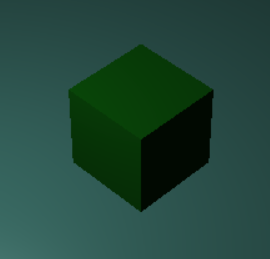
\includegraphics[scale=1.0]{images/ChMSAA/AnExampleOfAliasing.png}
    \caption{An example of aliasing}
    \label{fig::AliasingExample}
\end{figure}

\subsection{MSAA}

During rendering, we have determined a pixel's color based on a single sample
point placed at the center of the target pixel.
In this case, if the geometry doesn't cover the sample point, the entire pixel
is left blank.
This is the cause of aliasing.

\begin{figure}[H]
    \centering
    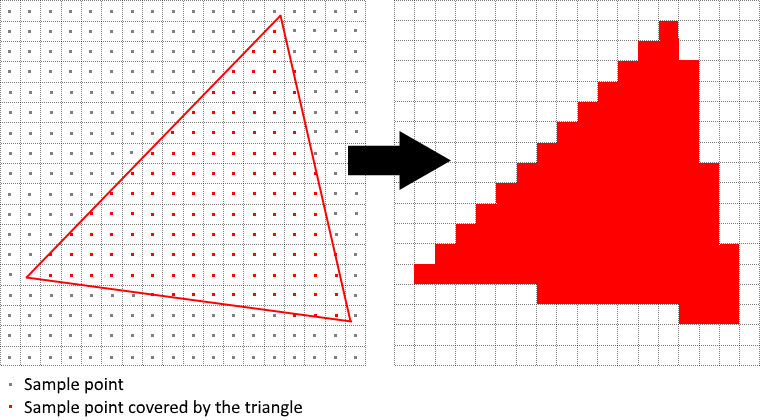
\includegraphics[scale=0.6]{images/ChMSAA/OneSamplePerPixel.png}
    \caption{Rendering taking one sample per pixel}
    \label{fig::OneSamplePerPixel}
\end{figure}

\begin{figure}[H]
    \centering
    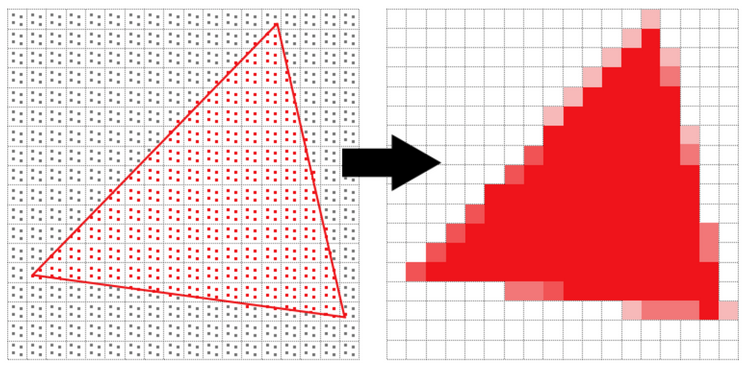
\includegraphics[scale=0.62]{images/ChMSAA/FourSamplesPerPixel.png}
    \caption{Rendering taking four samples per pixel}
    \label{fig::FourSamplesPerPixel}
\end{figure}

MSAA uses multiple sample points per pixel to determine its final color.
More samples lead to better results but also mean more overhead.
For each pixel, the less samples are covered by the triangle, the less
the triangle color contributes to the pixel color.
In this way, edges are now surrounded by colors slightly lighter than the
edge's color.
This causes the edge to appear smooth when viewed from a distance.

\section{Adding MSAA In Vulkan}

Now that we have discussed what is MSAA, we can go on and add it to our
Vulkan application.

\subsection{Get Available Sample Count}

To start, we must determine how many samples our hardware can use.
To do this we determine the maximum number of samples for both color and
depth values.
Then we simply pick the highest sample count that both support.

\begin{minipage}{\linewidth}{\noindent}
    \lstinputlisting[
        language=C++,
        caption={Determine the maximum supported sample count},
        label={lst::GetMaxMSAASampleCount}
        ]{src/ChMSAA/GetMaxMSAASampleCount.cpp}
\end{minipage}

\subsection{Set Up Render Target}

Using MSAA, each pixel is sampled in an offscreen buffer which is then
rendered to the screen.
This buffer must be able to store more than one sample per pixel.
The problem is that we can't pass to the presentation engine a multisampled image.
Thus, before presenting we must resolve this buffer to another image that
stores one sample per pixel.
This image is the one that will actually be presented.

\subsubsection{Creating The Multisample Render Target}

Our new multisample render target is nothing but an image.
We have already seen how to create images using Vulkan.
The only thing different from before, is that we pass
a number of samples to our create image function.
Before we used the default value \texttt{VK\_SAMPLE\_COUNT\_1\_BIT}.

\begin{minipage}{\linewidth}{\noindent}
    \lstinputlisting[
        language=C++,
        caption={Create the multisample render target},
        label={lst::CreateMultisampleRenderTarget}
        ]{src/ChMSAA/CreateMultisampleRenderTarget.cpp}
\end{minipage}

\subsubsection{Update Depth Buffer Creation}

We also must update our depth buffer.
This is because it will also use multisampling.
We do this by simply passing \texttt{msaaSamples} to the create image
function.

\subsection{Update Render Pass}

Adding multisampling, we need to modify the render pass creation.
We set the color attachment and the depth attachment number of samples to
\texttt{msaaSamples}.
We also change the color attachment's final layout to
\texttt{VK\_IMAGE\_LAYOUT\_COLOR\_ATTACHMENT\_OPTIMAL}
We do this because multisampled images can't be directly presented.

\subsubsection{Add A Resolve Color Attachment}

We add a new color attachment to the render pass.
This attachment will be used for the resolve operations and
will be the one that will be passed to the presentation engine.

\begin{minipage}{\linewidth}{\noindent}
    \lstinputlisting[
        language=C++,
        caption={Color resolve attachment},
        label={lst::ColorResolveAttachment}
        ]{src/ChMSAA/ColorResolveAttachment.cpp}
\end{minipage}

\subsubsection{Render Pass Attchments}

Now our render pass has three attachments.

\begin{minipage}{\linewidth}{\noindent}
    \lstinputlisting[
        language=C++,
        caption={MSAA render pass attachments},
        label={lst::MSAARenderPassAttachments}
        ]{src/ChMSAA/MSAARenderPassAttachments.cpp}
\end{minipage}

\subsubsection{Update Color Subpass Description}

We must tell to our color subpass to actually use the color resolve attachment.
To do this we update its description.
We first create an attachment reference for the color resolve attachment.
Then, we set the color subpass' \texttt{pResolveAttachments} field
to a pointer to the color resolve attachment reference.

\begin{minipage}{\linewidth}{\noindent}
    \lstinputlisting[
        language=C++,
        caption={Color resolve attachment reference},
        label={lst::ColorResolveAttachmentReference}
        ]{src/ChMSAA/ColorResolveAttachmentReference.cpp}
\end{minipage}

\subsection{Update Multisampling Pipeline State}

Not only we need to create resources that are compatible for using MSAA.
We also need to directly enable it on the pipeline state object.

\begin{minipage}{\linewidth}{\noindent}
    \lstinputlisting[
        language=C++,
        caption={Enable multisampling},
        label={lst::MSAAPipelineMultisampleState}
        ]{src/ChMSAA/MSAAPipelineMultisampleState.cpp}
\end{minipage}

\subsection{Update Framebuffer}

During rendering, when we create a framebuffer, we must update
its attachments array.
We use the new render target we created earlier as the first attachment.
We use the depth buffer as the second attachment.
And we use the next swapchain image as the color resolve attachment.

\section{Side By Side Comparison}

Here we can see a side by side comparison of the image.
On the left we see the cube rendered without using MSAA.
On the right we see the cube rendered using MSAA.
As explained earlier, the jagged pattern gets blurred making it look
smoother.

\begin{figure}[H]
    \centering
    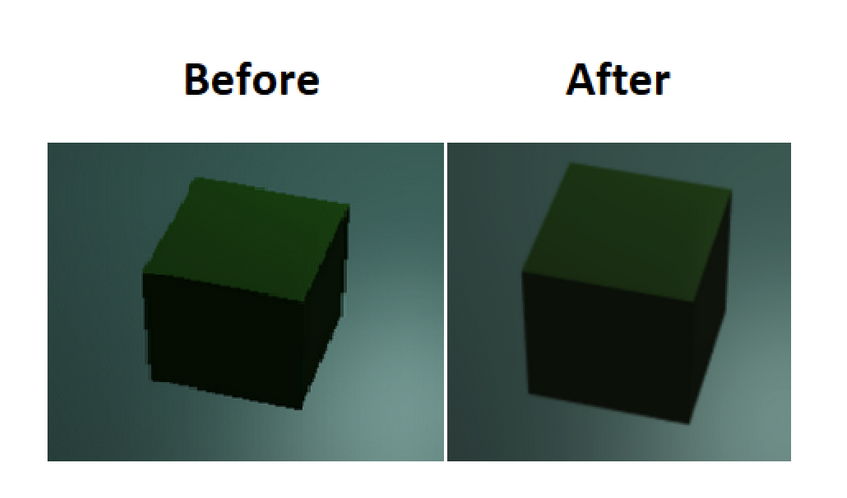
\includegraphics[scale=0.40]{images/ChMSAA/BeforeAfterMSAA.png}
    \caption{Before and after MSAA}
    \label{fig::MSAASideBySide}
\end{figure}
